\newchapter{Perspective}{Perspective: Summary \& Discussion}{Perspective: Summary \& Discussion}
\label{chapter:5}

In this chapter we summarize the work presented in this dissertation.  We follow this summary with a discussion of the challenges that must be overcome if merging clusters are to reach their true potential as dark matter probes and discuss potential solutions to these challenges.

\section{Dissertation Summary}

Over the past century our understanding of the Universe has undergone dramatic revisions which have culminated in accurate (percent level) measurements of the composition of the universe.
While the general scientific community agrees upon the composition of the universe, the properties of the bulk of this composition (dark matter and dark energy) remain a mystery.
This dissertation has presented our recent efforts to better understand the properties of dark matter (DM).

In Chapter \ref{chapter:1} we provided a brief review of the history of DM (\S\ref{section:DMhistory}), showing that while Fritz Zwicky provided the first evidence of DM in 1933 \citep{Zwicky:1933ub} it wasn't until the work of Vera Rubin and collaborators \citep{Rubin:1970gu} in the 1970's that DM garnered much attention.
Three general candidates for DM originally dominated the debate:
it was simply massive compact objects made up of standard model particles, or it was that it was some new particle, or it was that general relativity needed to be modified.
The MACHO experiment \citep{Alcock:2000bw} eventually ruled out the possibility that massive compact objects made up the bulk of DM, and merging galaxy clusters ruled out modified gravity \citep{Clowe:2006hr} thus providing strong evidence for DM being a new particle.
We reviewed the generally accepted cold dark matter (CDM) properties (\S\ref{section:CDMproperties}) but provided motivation for considering that DM might actually interact with itself other than through gravity (SIDM model; \S\ref{section:SIDMmotivation}).
We also reviewed the possible probes of SIDM (\S\ref{section:SIDMprobes}), highlighting  merging galaxy clusters (\S\ref{section:MergingClustersSIDMprobe}) and the four methods of constraining SIDM with observations of merging clusters.

In Chapter \ref{chapter:2} we introduced the the merging galaxy cluster DLSCL J0916.2+2951 (also known as the Musket Ball Cluster) and presented our multi-wavelength studies of the system.
Our photometric and spectroscopic observations show that the system consists of two subclusters separated by a projected distance of 1.0$\pm$0.1\,Mpc and a line-of-sight velocity difference of $v_{\rm los}=670^{+270}_{-330}$\,km\,s$^{-1}$.
Thus the two subclusters are close enough to be physically associated with one another.
Our weak lensing analysis of the north and south subclusters show that they have comparable mass ($1.7^{+2.0}_{-0.72}\times10^{14}$\,M$_\sun$  and $3.1^{+1.2}_{-0.79}\times10^{14}$\,M$_\sun$, respectively), suggesting that the system is a major merger.
Our Sunyaev-Zel'dovich effect and X-ray observations show that the cluster gas is located between the two subclusters proving that the Musket Ball Cluster is a post merger system where the collisional gas has become dissociated from the effectively collisionless galaxies and DM.
Thus the Musket Ball Cluster is an excellent candidate to constrain the DM self-interaction cross-section ($\sigma_{\rm SIDM}$).

In Chapter \ref{chapter:3} we discussed the importance of understanding the dynamic history of mergers when attempting to use them to constrain the properties of DM.
We developed a new Monte Carlo based method to discern the properties of dissociative mergers and propagate the uncertainty of the measured cluster parameters in an accurate and Bayesian manner.
We verified it against an existing hydrodynamic N-body simulation, and applied it to two known dissociative mergers: 1ES 0657-558 (Bullet Cluster) and the Musket Ball Cluster.
We find that the dynamic properties of the Musket Ball occupy a significantly different volume of merger phase space than the Bullet Cluster.
The Musket Ball Cluster, being $3.4^{+3.8}_{-1.4}$ times further progressed than the Bullet Cluster, could potentially provide tighter constraints on $\sigma_{\rm DM}$ since the offset between galaxies and dark matter should initially increase with time post-merger for  $\sigma_{\rm DM}>0$.

In Chapter \ref{chapter:4} we compared the locations of the galaxies, gas, and DM in the Musket Ball Cluster to provide insight into the properties of DM.
We constrain the central gas distribution's projected centroid to within 9'' (57\,kpc at $z$=0.53), see \S\ref{section:GasLocation}.
Using both the extensive spectroscopic and photometric redshifts we constrain the galaxy centroid of the northern subcluster to within 5.3" (33\,kpc at $z$=0.53) and the galaxy centroid of the southern subcluster to within 3.3" (21\,kpc at $z$=0.53), see \S\ref{section:GalaxyLocation}.
And using our tomographic WL method applied to the HST measured shapes we constrain the projected WL centroid of the northern subcluster to within 13'' (82\,kpc at $z$=0.53) and the WL centroid of the southern subcluster to within 11'' (69\,kpc at $z$=0.53), see \S\ref{section:WLLocation}.
Our measurement of a significant offset of the gas between the DM in each subcluster enabled us to achieve the constraint $\sigma_{\rm DM} m_{\rm DM}^{-1} \lesssim 7$\,cm$^2$\,g$^{-1}$.
Given the dependence on the surface mass density of this method it is not surprising that this constraint is less than that achieved with more massive mergers \citep{Markevitch:2004dl, Bradac:2008gw, Merten:2011gu}.
Finally in this chapter we investigated the galaxy-WL offset, since if DM self-interacts then the effectively collisionless galaxies might be expected to lead the DM post-merger.
While we find that the galaxies appear to be leading the WL centroid in the southern subcluster by $\sim$20.5'' (129\,kpc at $z$=0.53), see \S\ref{section:GalaxyWLOffset}, this only provides $\sim$85\% confidence that $\sigma_{\rm DM}>0$.
Furthermore, when we account for the observation that the galaxy centroid appears to trail the WL centroid in the northern subcluster by $\sim$7.4'' (47\,kpc at $z$=0.53), the confidence that $\sigma_{\rm DM}>0$ falls to $\sim$55\%.
While the SIDM scenario is slightly preferred over the CDM scenario it is not significantly so.
SIDM simulations of the Musket Ball Cluster are needed to turn these observations into quantitative constraints on $\sigma_{\rm DM}$.


\section{Discussion on the Path Forward}

There are a number of outstanding uncertainties/challenges that must be overcome before merging clusters are proven capable of obtaining the necessary SIDM constraints to either measure $\sigma_{\rm DM}$ or constrain it to the point of being astrophysically uninteresting.

\subsection{Uncertainty in the Location of Galaxies and DM/Lensing}

Perhaps the most notable challenge is related the results from the recent theoretical studies of SIDM effects in merging clusters by \citet{Kahlhoefer:2013wp} (which were presented in the arXiv one week before the completion of this dissertation).
There are a number of promising results from their study which support claims made previously in this dissertation (e.g., they confirm the expectation that the galaxy-DM offset increases following the merger, and also confirm that for some models of DM, common mergers such of the Musket Ball Cluster can have more constraining power than extreme mergers such as the Bullet Cluster).
However, one result from their study casts doubt on the possible effectiveness of merging galaxy clusters to constrain SIDM.
In particular, they find that the typical galaxy-DM offset ranges between $\sim$5--15\,kpc for allowable ranges of $\sigma_{\rm DM}$.
This is much smaller than the galaxy and WL centroid uncertainties typically measured for galaxy clusters ($\sim$20--100\,kpc).
And since most mergers don't occur directly in the plane of the sky, the observable projected offset will be $\lesssim5$--15\,kpc, assuming the \citet{Kahlhoefer:2013wp} results are correct.
Even disregarding intrinsic scatter of the galaxy-DM location and systematic offset effects due to the dissociated gas and other subcluster mass, it will take a large number of dissociative mergers to reach the $\sim$10\,kpc offset level.
Take for example the Musket Ball Cluster studied in this dissertation.
We find that we are able to constrain the galaxy centroid in each subcluster to $\sim\pm$25\,kpc and the WL centroid in each subcluster to $\sim\pm$70\,kpc.
This roughly translates to a centroid offset uncertainty of $\sigma_{\rm offset}\sim$80\,kpc (again for argument's sake disregarding other systematic offset errors).
Since the offset measurement is largely Poisson noise dominated (i.e. $\sigma_{\rm offset}\propto N^{-1/2}$), it will take roughly 14--128 dissociative mergers\footnote{Assuming that two centroid offset measurements can be made for each dissociative merger, since there are two subclusters per dissociative merger.} similar to the Musket Ball Cluster to achieve the necessary centroid accuracy of $\lesssim$5--15\,kpc.
While this example is highly simplified, and it is not clear how general or accurate the \citet{Kahlhoefer:2013wp} results are,  it does highlight the magnitude of this challenge and the importance of investigating it further.

Along these lines, the intrinsic scatter between the location of the galaxies and DM in galaxy clusters is still not accurately known.
If the intrinsic scatter is of order the centroid measurement uncertainty then this will add significantly to the challenge of constraining SIDM with the galaxy-WL offset measurement in dissociative mergers.
Two immediate means of constraining this intrinsic scatter is through studies of the scatter in existing simulations and observations of relaxed cluster systems, which should provide a lower limit on the expected scatter in merging systems.
A number of high resolution simulations of relaxed clusters exist \citep[e.g.][which include both CDM and SIDM simulations]{Peter:2012vi, Rocha:2012tr}.
By treating the subhalos in the cluster simulation as galaxies, one could estimate the intrinsic galaxy-DM offset.
Alternatively a purely observational approach could study the galaxy-lensing offset in a sample of well measured relaxed clusters.
For example the Cluster Lensing and Supernova Survey with Hubble (CLASH) galaxy cluster sample (20 relaxed clusters, $\sim$5--30\,M$_\sun$) provides excellent weak and strong lensing data to locate the DM as well as 16-band photometric redshifts to identify cluster members for the galaxy population location.
Researchers of the Merging Cluster Collaboration are pursuing both avenues.

\subsection{Find and study more dissociative mergers}

Regardless of the magnitudes involved in the intrinsic scatter of the galaxy-WL/DM offset, it will be important to study as many dissociative mergers as possible in order to reduce this noise.
Fortunately the number of confirmed dissociative mergers has been increasing at a rapid rate (see Figure \ref{figure:N_Mergers}).
Prior to 2013 all of the dissociative mergers were serendipitously discovered, often requiring photometric, spectroscopic, lensing and X-ray observations for identification.
The rapid rise in the number of confirmed mergers after 2013 is due to the radio relic selection method.
Radio selection is an efficient way to identify dissociative mergers because the shock produced by a merger results in a ``radio relic'' (uniquely diffuse emission in an arc around part of the cluster, e.g. van Weeren et al. 2010).
So rather than needing photometric, spectroscopic, lensing and X-ray observations it is possible to identify dissociative mergers with just radio observations.
Thus wide-area radio surveys can provide many candidates. 
NVSS has already found a few dozen, and LOFAR is projected to find about 1000 \citep{Nuza:2012fu}.
The Merging Cluster Collaboration has begun an extensive follow-up of these radio relic mergers (see the red points in Figure \ref{figure:N_Mergers} after 2013) with Keck spectroscopy, Subaru and HST imaging (archival and recently awarded: GO-13343, Co-PI Wittman, Co-PI Dawson), and Chandra and XMM X-ray imaging.

\begin{figure}
\centering
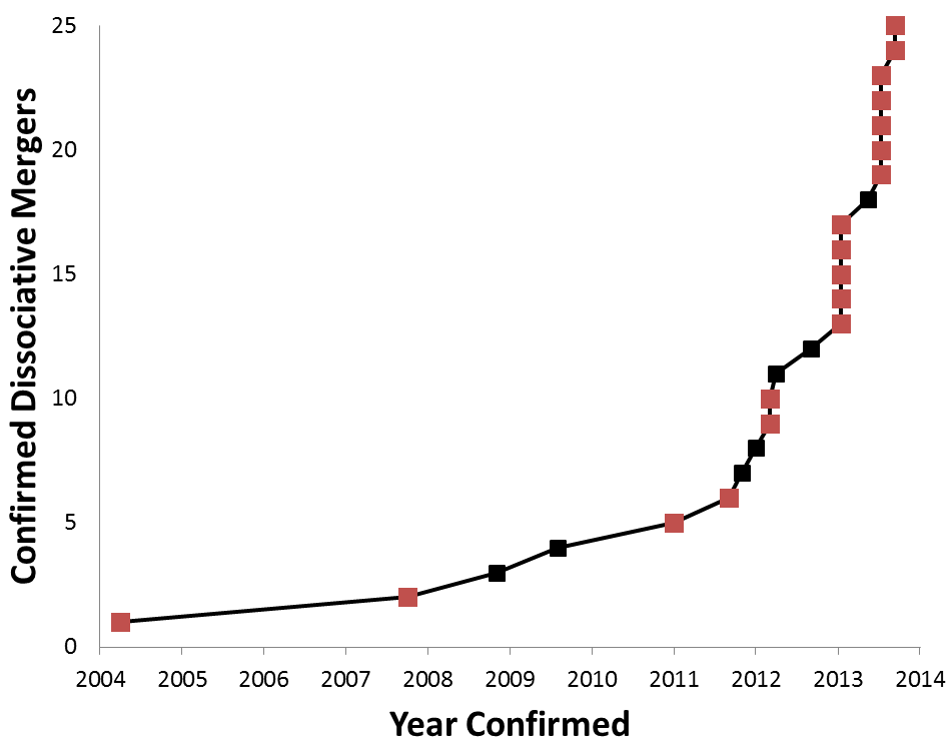
\includegraphics[width=4in]{Chapter5/NumberOfConfirmedDissociativeMergers.png}
\caption[Number of confirmed dissociative mergers as a function of time.]{
Number of confirmed dissociative mergers as a function of time.
The red points identify mergers that the Merging Cluster Collaboration are studying to  constrain the properties SIDM.
Up until 2013 dissociative mergers were all serendipitously discoveries.
The rapid rise in the number of confirmed mergers after 2013 is due to the radio relic selection method.
}
\label{figure:N_Mergers}
\end{figure}

Another promising avenue of dissociative merger discovery is with the optical-Sunyaev Zel'dovich effect identification method that led to the discovery of the Musket Ball Cluster.
Since the DES optical survey \citep{Collaboration:2005vv} will overlap much of the SPT \citep{Ruhl:2004io} and ACT \citep{Hincks:2010ff} Sunyaev-Zel'dovich effect (SZE) surveys it will be possible to search for significant offset of an SZE peak between a bimodal distribution of galaxies.
Based on the simulated and observed SZE cluster counts in the SPT survey \citep{Vanderlinde:2010hr, Song:2012tz} and the fraction of all clusters that are dissociative mergers \citep{ForeroRomero:2010cc} we estimate that $\sim$50 detectable dissociative mergers will be observed in the 4000 degree$^2$ SPT-DES survey.  Selection bias will result in mergers with large mass (i.e., better signal-to-noise) and large projected separations (i.e., later stage mergers where the expected DM-galaxy offset is maximized).  These will potentially be some of the best dissociative mergers with which to constrain $\sigma_{\rm DM}$, although there is the potential disadvantage that these typically higher redshift clusters and their angular scales will be smaller.


Looking further into the future, the LSST optical survey \citep{Tyson:2002hn} will cover a larger area than DES and go much deeper.
When it is coupled with upcoming all-sky X-ray surveys (e.g., eROSITA), that will enable much better angular resolution of the gas compared to SPT and ACT, there is the possibility to discover thousands of dissociative mergers.
Additionally, LSST with have multi-band photometric redshifts and excellent lensing quality data.
Thus it is conceivable that the field of dissociative merger science will enter an era where the statistical errors no longer dominate the measurements. 

\subsection{Going from Observations to Dark Matter Constraints}

Beyond the challenges associated with making the galaxy-DM offset measurement there remains the challenge of translating that measurement into a constraint on $\sigma_{\rm DM}$.
This challenge has both an observational element and a theoretical element.

Observationally it is possible to measure the projected galaxy-DM offset but this needs to be translated into a three-dimensional offset.
As noted in Chapter \ref{chapter:3}, there are severe limitations in our ability to do this, largely due to the difficulty in constraining the angle of the merger axis with respect to the plane of the sky ($\alpha$).
With just the commonly available measurements of the subclusters (mass, relative velocities along the line of sight, and projected separation) the magnitude of the three-dimensional distance errors often exceeds the actual distances being measured (see e.g.\,$d_{\rm 3D}$ of Tables \ref{bulletresultparam} and \ref{musketballresultparam}).
This is potentially a serious problem since there is only a factor of $\sim$2--4 difference between the expected galaxy-DM offset of different $\sigma_{\rm DM}$ models \citep{Markevitch:2004dl, Kahlhoefer:2013wp}.
Fortunately though, moderate constraints on $\alpha$ can translate to significant constraints on 
$d_{\rm 3D}$.
Take for example the Bullet Cluster with the added temporal prior (\S\ref{sec_addedprior}) where a factor of two improvement on the $\alpha$ uncertainty was accompanied by a factor of 9 improvement on the $d_{\rm 3D}$ uncertainty.
An added advantage of our radio relic sample is that radio polarization measurements of the radio relic can place an upper limit on $\alpha$ \citep{Ensslin:1998tx}, for example in the case of CIZA J2242.8+5301 the polarization measurements translated to an upper limit on $\alpha$ of 30\,degrees.
Thus it is conceivable that this element of the challenge is not a daunting as it might seem.

The other major element of the challenge of translating the galaxy-DM measurement into a constraint on $\sigma_{\rm DM}$ is theoretically predicting the galaxy-DM offset for a given $\sigma_{\rm DM}$.
\citet{Randall:2008hs} showed that a promising technique is simulating a merger with collisionless ``galaxy'' particles and DM particles with varying $\sigma_{\rm DM}$ between runs.
However there were a number of simplifying assumptions in their simulations that must be addressed if dissociative mergers are going to accurately constrain $\sigma_{\rm DM}$: 

\textit{(i)} They only modeled a single analog of the Bullet Cluster. 
By only choosing to model one analog of the Bullet Cluster, that albeit was representative of the most likely observed subcluster masses and projected separation, they failed to propagate the uncertainty in the observed merger parameters to the uncertainty in the expected offset for a given $\sigma_{\rm DM}$; thus the lack of uncertainty estimates in there expected offset results.

\textit{(ii)} The collision velocity in their simulation is extremely high.
They based their choice of collision velocity on the Mach number of the gas shock feature, but as noted in Chapter \ref{chapter:3} there are physical reasons this velocity is an overestimate of the true relative velocity.
This resulted in an overestimate of the expected offset.
	
\textit{(iii)} The galaxies were uniformly distributed in the DM halo and they used an unreasonably large number of galaxy particles. 
This unrealistic assumption fails to account for the intrinsic scatter related to the Poisson noise associated with the galaxies (see \S\ref{section:GalaxyLocation}).

\textit{(iv)} Galaxies were not embedded in their own DM subhalos.
This could affect the expected offset between the galaxies and the cluster DM halo. The DM subhalos will experience a drag force due to  $\sigma_{\rm DM}$, and this will be translated to some degree into a gravitational drag force on the galaxies due to the gravitational dominance of the subhalos on small scales. 

\textit{(v)} The central densities of the subclusters were unphysically cuspy for the chosen $\sigma_{\rm DM}$.
As \citet{Rocha:2012tr} found the central density of SIDM halos becomes cored as $\sigma_{\rm DM}$ increases.
Since the interaction rate scales roughly as the SIDM density squared, using King profiles for all the halos can result in overestimates of the expected offset. 

At the heart of problems \textit{i}--\textit{iv} is the fact that the simulations failed to take into account the wealth of cosmological prior information.
One possible solution to this and all of the associated problems is identifying likely merger analogs in large cosmological N-body simulations rather than setting up a simplified toy model of the merger.
And then resimulating these analogs at higher resolution with varying $\sigma_{\rm DM}$.
Perhaps the best means of identifying analog mergers is through importance sampling. 
Where the known properties of merger in the cosmological simulation are cast in terms of the observable properties (subcluster masses, relative line-of-sight velocity, and projected separation), then given the PDF's of the observed properties a likelihood of each simulated analog can be calculated.
Because each simulated analog of the observed merger will have an associated likelihood, we could then create a posterior PDF of the expected galaxy-DM offset for a given $\sigma_{\rm DM}$ that marginalizes over all other uncertainties associated with a given merger.
It will then be possible to combine the $\sigma_{\rm DM}$ constraints in a fair and well defined manner from an ensemble of dissociative mergers and reduce the noise associated with the galaxy-DM offset constraint method.

\section{Concluding Remarks}

The work of this dissertation has highlighted the promise that merging galaxy clusters offer to either measure $\sigma_{\rm DM}$ or constrain it to the point of being astrophysically uninteresting.
It has also highlighted the many challenges that must be overcome before this promise can be realized.
This is an exciting time as the merging galaxies cluster science will face most these challenges within the next couple years.
While we may not have any definitive results on SIDM in this time, we will have definitively assessed the value of merging galaxy clusters as probes of SIDM.

%\bibliographystyle{apj}
%\bibliography{Chapter1/chapter1}{}



%% The References
%\bibliographystyle{thesis}
%\begin{singlespacing}
%  \bibliography{Chapter3/chapter3}
%\end{singlespacing}
